\documentclass[10pt]{article}

\title{Term project report}
\newcommand{\course}{CS 555: Data Science}

\author{Sasha Malone}

\usepackage[xetex]{graphicx} % allow embedded images
  \setkeys{Gin}{width=\linewidth,totalheight=\textheight,keepaspectratio}
  \graphicspath{{graphics/}} % set of paths to search for images
  \usepackage{adjustbox}
\usepackage{amsmath}  % extended mathematics
\usepackage{amssymb}  % extended mathematics
\usepackage{mathtools}
\usepackage{amsthm}   % theorem styles
\usepackage{booktabs} % book-quality tables
\usepackage{units}    % non-stacked fractions and better unit spacing
\usepackage{multicol} % multiple column layout facilities
% \usepackage{fullpage} % reduce margins
\usepackage[margin=1in,tmargin=0.7in,includehead,includefoot,headheight=12pt,heightrounded]{geometry}

\usepackage{hyperref}

\usepackage{lmodern}
\usepackage{xcolor}
\usepackage{listings}
\usepackage{fancyhdr}
\pagestyle{fancy}

\makeatletter
\lhead{\course \\ \vspace{1pt} \large \@title}
\rhead{\textit{\today} \\ \vspace{1pt} \large \@author}
\makeatother

\usepackage{enumerate}

\usepackage{titlesec}
\colorlet{punct}{red!60!black}
\definecolor{background}{HTML}{EEEEEE}
\definecolor{delim}{RGB}{20,105,176}
\colorlet{numb}{magenta!60!black}

\lstdefinelanguage{json}{
    basicstyle=\normalfont\ttfamily,
    showstringspaces=false,
    breaklines=true,
    literate=
     *{:}{{{\color{punct}{:}}}}{1}
      {,}{{{\color{punct}{,}}}}{1}
      {\{}{{{\color{delim}{\{}}}}{1}
      {\}}{{{\color{delim}{\}}}}}{1}
      {[}{{{\color{delim}{[}}}}{1}
      {]}{{{\color{delim}{]}}}}{1},
}


\usepackage{fontspec}
\setmainfont{Century Expanded Regular.otf}[
    Path =  /usr/share/fonts/OTF/,
    BoldFont = Century Expanded Bold.otf,
    ItalicFont = Century Expanded Italic.otf
]
\makeatletter
\renewcommand{\maketitle}{\bgroup\setlength{\parindent}{0pt}
    \begin{center}
    \LARGE \textbf{\@title}
    % \vspace{1pt}
    % \large \textit{\@author \quad $\vert$ \quad \course \quad $\vert$\quad \@date}
    \end{center}
\egroup
}
\makeatother

% Standardize command font styles and environments
\newcommand{\doccmd}[1]{\texttt{\textbackslash#1}}% command name -- adds backslash automatically
\newcommand{\docopt}[1]{\ensuremath{\langle}\textrm{\textit{#1}}\ensuremath{\rangle}}% optional command argument
\newcommand{\docarg}[1]{\textrm{\textit{#1}}}% (required) command argument
\newcommand{\docenv}[1]{\textsf{#1}}% environment name
\newcommand{\docpkg}[1]{\texttt{#1}}% package name
\newcommand{\doccls}[1]{\texttt{#1}}% document class name
\newcommand{\docclsopt}[1]{\texttt{#1}}% document class option name
\newenvironment{docspec}{\begin{quote}\noindent}{\end{quote}}% command specification environment

\newtheorem{thm}{Theorem}
\theoremstyle{definition}
\newtheorem{defn}{Definition}
\newtheorem{exer}{Exercise}
\newtheorem*{exer*}{Exercise}
\theoremstyle{remark}
\newtheorem*{soln}{Solution}
\newtheorem*{remark}{Note}

\newcommand{\ds}{\displaystyle}
\renewcommand{\geq}{\geqslant}
\renewcommand{\leq}{\leqslant}

\providecommand{\tightlist}{%
      \setlength{\itemsep}{0pt}\setlength{\parskip}{0pt}}

\DeclarePairedDelimiter{\abs}{\lvert}{\rvert}
\DeclarePairedDelimiter{\inner}{\langle}{\rangle}
\DeclarePairedDelimiter{\norm}{\lVert}{\rVert}

\begin{document}

\emph{NB:} As the total filesize of my data and project code exceeds
Blackboard's upload limit, please note that it is publicly available on Github
at URL \texttt{http://github.com/sverona/meleeWHR}. Partial replication
instructions are available in the repository's readme file.

\hypertarget{background-and-problem-description}{%
\section{Background and problem description}\label{background-and-problem-description}}

\emph{Super Smash Bros.~Melee}, a fighting game
originally released in 2001, has recently experienced a resurgence in
competitive play. Major tournament series such as Genesis and Evolution
regularly attract upwards of 1,000 entrants {[}1{]}, a scale otherwise
unheard of for decade-old games incapable of online play.

Melee It On Me (\emph{MIOM}), the competitive community's primary
governing body, produces annual ranking lists of the 100 most skilled
players, established by panel vote. While the general accuracy of these
lists is widely accepted, both the placement of individual players and
the rankings' general methodology are highly debated within the community
at large. There have been many attempts at using existing rating systems such
as Elo and Glicko to generate comparable rankings, but few are still
publicly maintained, partially due to the scattered nature of the
available data. Further, these rankings (like their MIOM counterparts)
are produced at infrequent intervals from aggregated resuls. Thus, since
the scene lacks a formal competitive circuit, the task of ranking the
top players attending an upcoming tournament (e.g., for seeding
purposes) falls mainly on that tournament's organizers.

\hypertarget{objectives}{%
\section{Objectives}\label{objectives}}

The goals of this project were to

\begin{enumerate}
\def\labelenumi{\roman{enumi}.}
\tightlist
\item
  consolidate the available tournament data, dating as far back as
  2003-4, into a publicly maintained dataset;
\item
  use this dataset and a maximum-likelihood estimation method such as
  Whole-History Rating (\emph{WHR}) {[}2{]} to reconstruct real-time
  ratings for the period comprising the earliest modern tournaments in
  2004-5 to the present day;
\item
  use D3.js {[}3{]} to visualize these time-series in a manner similar
  to {[}4{]}.
\end{enumerate}

Items (i) and (ii) were completed to some degree of satisfaction. Item
(iii) was accomplished through Matplotlib (see appendix.) Visualization
using D3.js remains a future goal (see Section 6.4.)

\section{Overview of methodology and research question}
The primary question of interest is to derive a stable measure of player
skill from the sequence of match records. One method of doing so that
has been adopted by other e-sports communities is TrueSkill {[}5{]},
which assumes that player skill before any given match follows a
Gaussian distribution. The probability of one player defeating another
is then roughly approximated by the probability that a randomly sampled
value from the former's distribution exceeds one from the latter's; this
gives rise to the \emph{Bradley-Terry model}
\begin{align*}
    P_t(i > j) \approx \frac{\mu_{it}}{\mu_{it} + \mu_{jt}},
\end{align*}
where $\mu_{it}, \mu_{jt}$ are the means of players $i$ and $j$'s
distributions at time $t$. The TrueSkill algorithm, like many others,
performs maximum-likelihood estimation of these parameters using this
assumption. One goal of this project is to adapt this algorithm slightly
to model some of the peculiarities of \emph{SSBM}'s competitive
environment, as demonstrated, e.g., in {[}6{]}.

The WHR algorithm differs from TrueSkill in that it performs MLE retroactively
over the player's entire rating history (hence the name.) However, the
mathematics is similar; [5] gives a whole-history extension of TrueSkill that,
according to [2], produces similar results to WHR.

Ratings were interpolated using the following formula given in [2]; if the
mean of a player's skill distribution at time $t$, $\mu_t$, is to be interpolated
from the values $\mu_{t_1} = \mu_1$ and $\mu_{t_2} = \mu_2$, then we have
\begin{align*}
    \mu_t = \frac{\mu_1(t_2 - t) + \mu_2(t - t_1)}{t_2 - t_1}.
\end{align*}

\hypertarget{basic-data-model-and-project-workflow}{%
\section{Data cleaning}\label{basic-data-model-and-project-workflow}}

The data consists primarily of match metadata from tournament brackets,
as shown in the sample below at left. This data was sourced from Liquipedia [7][8],
using a scraper written in Python, and cleaned and reformatted into JSON, as
in the sample below at right. It contains the match data from a set between
top-level players at the tournament Shine 2017.

\lstset{frame=single,
        basicstyle=\small\ttfamily,
        basewidth=0.5em,
        breaklines=true,
        postbreak=\mbox{\textcolor{red}{$\hookrightarrow$}\space}
    }
\begin{figure}[!ht]
    \begin{minipage}[t][][t]{.46\textwidth}
        \begin{lstlisting}
|l1m3p1=S2J |l1m3p1flag=us |l1m3p1score=3
|l1m3p2=HugS |l1m3p2flag=us |l1m3p2score=1
|l1m3win=1
|l1m3p1char1=cf |l1m3p2char1=samus |l1m3p1stock1=0 |l1m3p2stock1=1 |l1m3win1=2 |l1m3stage1=Yoshi's Story
|l1m3p1char2=cf |l1m3p2char2=samus |l1m3p1stock2=1 |l1m3p2stock2=0 |l1m3win2=1 |l1m3stage2=Pokémon Stadium
|l1m3p1char3=cf |l1m3p2char3=samus |l1m3p1stock3=2 |l1m3p2stock3=0 |l1m3win3=1 |l1m3stage3=Yoshi's Story
|l1m3p1char4=cf |l1m3p2char4=samus |l1m3p1stock4=3 |l1m3p2stock4=0 |l1m3win4=1 |l1m3stage4=Yoshi's Story
|l1m3date=August 26, 2017
|l1m3details={{BracketMatchDetails|reddit=|comment=|vod=https://www.youtube.com/watch?v=7zTSvNM-E1c}}
        \end{lstlisting}
    \end{minipage} \hfill
    \begin{minipage}[t][][t]{.5\textwidth}
        \begin{lstlisting}[language=json]
"l1m3": {
    "date": "August 26, 2017",
    "details": {
        "comment": "",
        "reddit": "",
        "vod": "https://www.youtube.com/watch?v=7zTSvNM-E1c"
    },
    "p1": "S2J",
    "p1char1": "cf", "p1char2": "cf", "p1char3": "cf", "p1char4": "cf",
    "p1flag": "us",
    "p1score": "3",
    "p1stock1": "0", "p1stock2": "1", "p1stock3": "2", "p1stock4": "3",

    "p2": "HugS",
    "p2char1": "samus", "p2char2": "samus", "p2char3": "samus", "p2char4": "samus",
    "p2flag": "us",
    "p2score": "1",
    "p2stock1": "1", "p2stock2": "0", "p2stock3": "0", "p2stock4": "0",

    "stage1": "Yoshi's Story", "stage2": "Pok\u00e9mon Stadium", "stage3": "Yoshi's Story", "stage4": "Yoshi's Story",

    "win": "1",
    "win1": "2", "win2": "1", "win3": "1", "win4": "1"
}
        \end{lstlisting}
    \end{minipage}
\end{figure}

The resulting JSON data was sufficiently flexible to be input into the WHR
algorithm. Further applications of this dataset may require the imposition
of a relational schema.

\subsection{Relevant source code}
The raw bracket data is stored in the directory \texttt{brackets/}. Data
formatted as Wikitext (above left) has the extension \texttt{*.wiki}, while
data stored as JSON has the extension \texttt{*.wiki.json}.

The Liquipedia scraper is located at \texttt{scrape\_brackets.py}; the
Wikitext-to-JSON parser is located at \texttt{parse\_wikitext.py}.

\section{Results}
The computed ratings are stored in a JSON file and plotted using Matplotlib
(see the appendix.) The pertinent source code is located at \texttt{list\_top\_players.py}.

\subsection{Evaluation}
This section compares the results output by WHR at the end of each year from
2004 to 2016 with those compiled by MIOM (from 2013 to 2016) or by the
RetroSSBMRank panel (from 2004 to 2012.) The algorithm's precision, recall,
and $F_1$-score is evaluated for the top 10 (for Retro rankings) or top 25
(for MIOM rankings) players as evaluated by the foregoing source. For Retro
rankings, if an honorable mention was predicted within the top 10, it was
counted as one-half of a false positive. Detailed tables are included as an
appendix.

\begin{table}[!ht]
    \centering
\begin{tabular}{lllllll}
    \textbf{Period} & \textbf{TP} & \textbf{FP} & \textbf{FN} & \textbf{Precision} & \textbf{Recall} & $\mathbf{F_1}$ \textbf{score} \\
    2004            & 8           & 2           & 2           & 80\%               & 80\%            & 80\%    \\
    2005            & 7           & 2.5         & 3           & 73.68\%            & 70\%            & 71.79\% \\
    2006            & 6           & 3.5         & 4           & 63.16\%            & 60\%            & 61.54\% \\
    2007            & 7           & 3           & 3           & 70\%               & 70\%            & 70\%    \\
    2008            & 6           & 2.5         & 4           & 70.59\%            & 60\%            & 64.86\% \\
    2009            & 7           & 1.5         & 3           & 82.35\%            & 70\%            & 75.68\% \\
    2010            & 8           & 1.5         & 2           & 84.21\%            & 80\%            & 83.72\% \\
    2011            & 8           & 2.5         & 4           & 76.19\%            & 66.67\%         & 71.11\% \\
    2012            & 7           & 2.5         & 3           & 73.68\%            & 70\%            & 71.79\% \\
    2013            & 20          & 5           & 5           & 80\%               & 80\%            & 80\%    \\
    2014 Summer     & 20          & 5           & 5           & 80\%               & 80\%            & 80\%    \\
    2014            & 20          & 5           & 5           & 80\%               & 80\%            & 80\%    \\
    2015 Summer     & 19          & 6           & 6           & 76\%               & 76\%            & 76\%    \\
    2015            & 20          & 5           & 5           & 80\%               & 80\%            & 80\%    \\
    2016            & 20          & 5           & 5           & 80\%               & 80\%            & 80\%    \\
\end{tabular}
\end{table}

The performance is consistently around 75 percent, except in 2006 and 2008. Explanations for these can be found in Section 6.1 below. During the MIOM years, the algorithm's false positives were repeatedly drawn from the same set of six to seven international and inactive players, which MIOM explicitly disconsidered due to a lack of pertinent data. Were these players discarded from the WHR rankings, precision would improve to as much as 92 percent (in 2014.)

These ratings accord with a loose overview of Melee history. Setting the above table's findings aside, the magnitude of
the ratings attained by the ``Five Gods'' (Hungrybox, Armada, Mango, Mew2King, and PPMD) through the period around 2010 to 2015 provide a clear picture of their dominance over the competition; during this period, with few exceptions, one of the Five Gods won every event at which at least two were in attendance. Also visible are the player Ken's early dominance from approximately 2004 to 2006 and the rapid rise of the ``godslayers'' Leffen and Plup, the only two players to have defeated all Five Gods. The player Wobbles, who has defeated four of the five (all except Armada,) also makes a visible peak around 2012 to 2013.

\section{Directions for further improvement}

\subsection{Better missing value interpolation}
The primary shortcoming of this project is its total ignorance of tournaments
for which the brackets have been lost to history, but for which the
rank-order placement data survives. Many such events fall between 2003 and
2006, during the competitive scene's so-called ``stone age'' and ``golden
age.'' Both periods predated widespread use of tournament tracking software
(brackets were kept on paper, etc.) This partially explains the lower
performance in those years; the RetroSSBMRank panelists compiled those
rankings using data not currently available to the algorithm.

\par Adding these results to the dataset will require some form of
interpolation to approximate each player's path through the bracket. For
example, the round in which each player was eliminated can be determined
purely from the rank-order data. Working backward from this, Monte
Carlo methods can be used to obtain an approximation of the mean strength of
each bracket round. Then, each entrant's approximate bracket path can be
represented by victories or losses against a ``dummy'' player of each round's
approximate skill. This may bias the variance of the WHR estimates downward,
leading to imprecise future estimates, but this inaccuracy is minor compared
to the ones stemming from the current absence of this data.

\subsection{Further data gathering and reconstruction}
Many other events have bracket data that is either not publicly available or
in a different format (e.g., XML documents generated by tournament software
that have not been parsed and assimilated by Liquipedia.) Thus, there are
several major tournament brackets, most prominently the 2007 tournament known
as MELEEFC-Diamond, that can largely be reconstructed from available data.
However, tracking this data down will require reaching out to those
tournaments' organizers (and in some cases, entrants) individually, and as
such entail a time commitment outside the scope of a semester project.

\subsection{More robust data model}
Although JSON is probably sufficient for most small-scale applications of this
dataset, the current data model is the minimal viable one for this project.
Refactoring to support interpolated brackets, unknown match data, implementation
of further features such as stage and character choice, etc. may be of interest.

\subsection{Visualization and web application}
A plot of all players' ratings over time that has more interactive visual aids (e.g.,
highlighting of a moused-over time series,) will improve the usability of these
results. I plan to implement this using D3.js. On a longer-term scale, I would like
to transfer the data I have into a webapp that provides individual match data
richer than any single current source.

\subsection{Comparison with other ranking algorithms}
It is possible that the performance of this algorithm is eclipsed by simpler Elo-based
systems, contrary to the findings presented in [2]. However, the problems presented
in Section 6.1 make an objective comparison difficult. Further, as WHR encapsulates
many simpler Elo-based systems as special cases [2], this is an unlikely premise
in any case.

\newpage

\begin{thebibliography}{7}
\bibitem{size} https://www.ssbwiki.com/List\_of\_largest\_Smash\_tournaments
\bibitem{whr} https://www.remi-coulom.fr/WHR/WHR.pdf 
\bibitem{d3} https://d3js.org/
\bibitem{abacaba} https://www.youtube.com/watch?v=z2DHpW79w0Y
\bibitem{ttt} https://papers.nips.cc/paper/3331-trueskill-through-time-revisiting-the-history-of-chess.pdf
\bibitem{lua} https://www.reddit.com/r/SSBM/comments/4pitia/an\_objective\_ranking\_system\_that\_compensates\_for/
\bibitem{liquid} http://liquipedia.net/smash/Main\_Page
\bibitem{data} http://liquipedia.net/smash/index.php?title=Shine/2017/Melee/Singles\_Bracket\&action=edit\&section=4
\end{thebibliography}

\section{Time-series plot of data}

\begin{center}
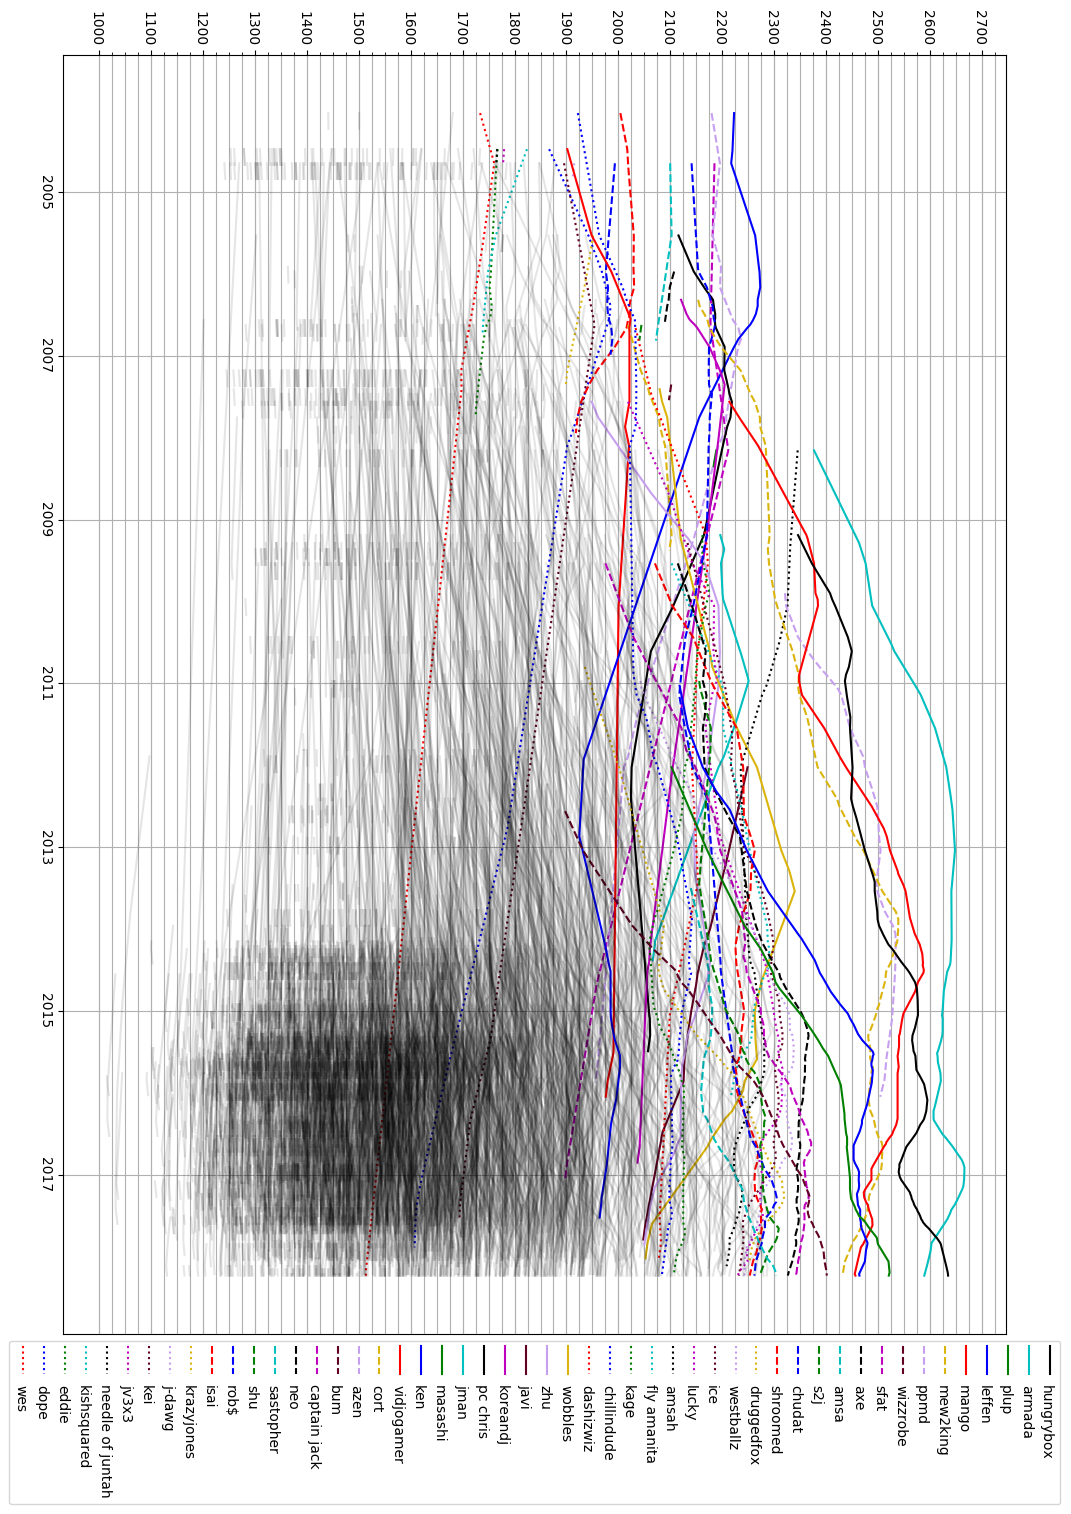
\includegraphics[width=.9\linewidth]{../plot-rotated.png}
\end{center}

\newpage
\section{RetroSSBMRank and Modern SSBMRank vs. WHR}
\begin{table}[!ht]
    \footnotesize

    \parbox{.33 \textwidth}{
        \centering
        \caption{2004}
\begin{tabular}{lcc}
    \textbf{Player} & \textbf{RetroRank} & \textbf{WHR Rank} \\
    Ken             & 1                      & 1        \\
    Captain Jack    & 2                      & 3        \\
    Azen            & 3                      & 2        \\
    Isai            & 4                      & 6        \\
    ChuDat          & 5                      & 4        \\
    Sastopher       & 6                      & 5        \\
    Wes             & 7                      & NR       \\
    Rori            & 8                      & NR       \\
    Chillindude     & 9                      & 8        \\
    Rob\$           & 10                     & 7        \\
    Vidjo           & NR                     & 9        \\
    J-Dawg          & NR                     & 10        \\
\end{tabular}
}
    \parbox{.33 \textwidth}{
        \centering
        \caption{2005}
\begin{tabular}{lcc}
    \textbf{Player} & \textbf{RetroRank} & \textbf{WHR Rank} \\
    Ken             & 1                      & 1        \\
    ChuDat          & 2                      & 4        \\
    Isai            & 3                      & 8        \\
    Azen            & 4                      & 2        \\
    Vidjo           & 5                      & 10       \\
    NEO             & 6                      & 6        \\
    Chillindude     & 7                      & 9        \\
    KrazyJones      & 8                      & 13       \\
    Caveman         & 9                      & 20       \\
    DieSuperFly     & 10                     & 22       \\
    PC Chris        & HM                     & 5        \\
    Captain Jack    & NR                     & 3        \\
    Sastopher       & NR                     & 7        \\
\end{tabular}
}
    \parbox{.33 \textwidth}{
        \centering
        \caption{2006}
\begin{tabular}{lcc}
    \textbf{Player} & \textbf{RetroRank} & \textbf{WHR Rank} \\
    Ken             & 1                      & 2        \\
    Azen            & 2                      & 1        \\
    PC Chris        & 3                      & 4        \\
    ChuDat          & 4                      & 7        \\
    KoreanDJ        & 5                      & 6        \\
    Mew2King        & 6                      & 3        \\
    Isai            & 7                      & 19       \\
    Vidjo           & 8                      & 15       \\
    Chillindude     & 9                      & 14       \\
    DieSuperFly     & 10                     & 22       \\
    NEO             & HM                     & 8        \\
    Captain Jack    & NR                     & 5        \\
    Sastopher       & NR                     & 9        \\
    DaShizWiz       & NR                     & 10       \\
\end{tabular}
}
    \parbox{.33 \textwidth}{
        \centering
        \caption{2007}
\begin{tabular}{lcc}
    \textbf{Player} & \textbf{RetroRank} & \textbf{WHR Rank} \\
    Mew2King        & 1                      & 1        \\
    Ken             & 2                      & 8        \\
    KoreanDJ        & 3                      & 6        \\
    PC Chris        & 4                      & 4        \\
    ChuDat          & 5                      & 7        \\
    Azen            & 6                      & 5        \\
    Chillindude     & 7                      & 16       \\
    Drephen         & 8                      & 33       \\
    Cort            & 9                      & 12       \\
    Mango           & 10                     & 2        \\
    Captain Jack    & NR                     & 3        \\
    Wobbles         & NR                     & 9        \\
    DaShizWiz       & NR                     & 10       \\
\end{tabular}
}
    \parbox{.33 \textwidth}{
        \centering
        \caption{2008}
\begin{tabular}{lcc}
    \textbf{Player} & \textbf{Retro Rank} & \textbf{WHR Rank} \\
    Mew2King        & 1                      & 4        \\
    Mango           & 2                      & 2        \\
    Cort            & 3                      & 17       \\
    Azen            & 4                      & 10       \\
    PC Chris        & 5                      & 7        \\
    ChuDat          & 6                      & 8        \\
    KoreanDJ        & 7                      & 6        \\
    HugS            & 8                      & 33       \\
    Ka-master       & 9                      & NR       \\
    Jman            & 10                     & NR       \\
    Armada          & HM                     & 1        \\
    Amsah           & HM                     & 3        \\
    Captain Jack    & HM                     & 5        \\
    Masashi         & NR                     & 9        \\
\end{tabular}
}
    \parbox{.33 \textwidth}{
        \centering
        \caption{2009}
\begin{tabular}{lcc}
    \textbf{Player} & \textbf{Retro Rank} & \textbf{WHR Rank} \\
    Mango           & 1                      & 3        \\
    Armada          & 2                      & 1        \\
    Hungrybox       & 3                      & 2        \\
    Mew2King        & 4                      & 6        \\
    DaShizWiz       & 5                      & 11       \\
    Jman            & 6                      & 7        \\
    Zhu             & 7                      & 8        \\
    Darkrain        & 8                      & 33       \\
    PC Chris        & 9                      & 22       \\
    PPMD            & 10                     & 5        \\
    Amsah           & HM                     & 4        \\
    Lucky           & HM                     & 9        \\
    Kage            & HM                     & 10       \\
\end{tabular}
}
    \parbox{.33 \textwidth}{
        \centering
        \caption{2010}
\begin{tabular}{lcc}
    \textbf{Player} & \textbf{RetroRank} & \textbf{WHR Rank} \\
    Hungrybox       & 1                      & 2        \\
    Mango           & 2                      & 4        \\
    Armada          & 3                      & 1        \\
    Mew2King        & 4                      & 5        \\
    PPMD            & 5                      & 3        \\
    Jman            & 6                      & 7        \\
    Amsah           & 7                      & 6        \\
    KirbyKaze       & 8                      & 22       \\
    Lucky           & 9                      & 12       \\
    Fly Amanita     & 10                     & 9        \\
    Zhu             & HM                     & 10       \\
    Ice             & NR                     & 8        \\
\end{tabular}
}
    \parbox{.33 \textwidth}{
        \centering
\caption{2011 (top 12)}
\begin{tabular}{lcc}
    \textbf{Player} & \textbf{RetroRank} & \textbf{WHR Rank} \\
    Armada          & 1                      & 1        \\
    Mango           & 2                      & 4        \\
    PPMD            & 3                      & 2        \\
    Hungrybox       & 4                      & 3        \\
    Mew2King        & 5                      & 5        \\
    Lovage          & 6                      & 30       \\
    Zhu             & 7                      & 16       \\
    Fly Amanita     & 8                      & 10       \\
    Shroomed        & 9                      & 7        \\
    Wobbles         & 10                     & 6        \\
    S2J             & 11                     & 15       \\
    Axe             & 12                     & 17       \\
    Amsah           & HM                     & 8        \\
    Ice             & HM                     & 9        \\
    Jman            & HM                     & 11       \\
    KirbyKaze       & NR                     & 12       \\
\end{tabular}
}
    \parbox{.33 \textwidth}{
        \centering
        \caption{2012}
\begin{tabular}{lcc}
    \textbf{Player} & \textbf{RetroRank} & \textbf{WHR Rank} \\
    Armada          & 1                      & 1        \\
    PPMD            & 2                      & 3        \\
    Mango           & 3                      & 2        \\
    Hungrybox       & 4                      & 4        \\
    Mew2King        & 5                      & 5        \\
    Wobbles         & 6                      & 6        \\
    KirbyKaze       & 7                      & 13       \\
    Zhu             & 8                      & 29       \\
    ChuDat          & 9                      & 22       \\
    Shroomed        & 10                     & 7        \\
    Fly Amanita     & HM                     & 8        \\
    Leffen          & NR                     & 9        \\
    Ice             & NR                     & 10       \\
\end{tabular}
}

\end{table}

\newpage
\begin{table}[!ht]
    \footnotesize
    
    \parbox{.35 \textwidth}{
        \centering
        \caption{2013}
\begin{tabular}{lcc}
    \textbf{Player} & \textbf{SSBMRank} & \textbf{WHR Rank} \\
    Mango           & 1                      & 2        \\
    Armada          & 2                      & 1        \\
    Mew2King        & 3                      & 3        \\
    PPMD            & 4                      & 4        \\
    Hungrybox       & 5                      & 5        \\
    Hax             & 6                      & 22       \\
    Shroomed        & 7                      & 19       \\
    Wobbles         & 8                      & 7        \\
    KirbyKaze       & 9                      & 16       \\
    SFAT            & 10                     & 17       \\
    Axe             & 11                     & 10       \\
    PewPewU         & 12                     & 21       \\
    Ice             & 13                     & 8        \\
    Leffen          & 14                     & 6        \\
    Ryan Ford       & 15                     & 40       \\
    Silent Wolf     & 16                     & 14       \\
    Javi            & 17                     & 27       \\
    Zhu             & 18                     & 31       \\
    S2J             & 19                     & 30       \\
    Lucky           & 20                     & 11       \\
    Fly Amanita     & 21                     & 9        \\
    ChuDat          & 22                     & 24       \\
    Westballz       & 23                     & 12       \\
    Taj             & 24                     & NR       \\
    Overtriforce    & 25                     & 18       \\
    Amsah           & NR                     & 13       \\
    Plup            & 27                     & 15       \\
    Gucci           & 65                     & 20       \\
    Flash           & NR                     & 23       \\
    Fuzzyness       & 59                     & 25       \\
\end{tabular}
}
    \parbox{.35 \textwidth}{
        \centering
        \caption{2014 Summer}
\begin{tabular}{lcc}
    \textbf{Player} & \textbf{SSBMRank} & \textbf{WHR Rank} \\
    PPMD            & 1                      & 4        \\
    Mango           & 2                      & 2        \\
    Mew2King        & 3                      & 5        \\
    Armada          & 4                      & 1        \\
    Hungrybox       & 5                      & 3        \\
    Leffen          & 6                      & 6        \\
    Hax             & 7                      & 17       \\
    Westballz       & 8                      & 12       \\
    Fly Amanita     & 9                      & 10       \\
    Shroomed        & 10                     & 22       \\
    SFAT            & 11                     & 18       \\
    aMSa            & 12                     & 33       \\
    Ice             & 13                     & 8        \\
    S2J             & 14                     & 29       \\
    Colbol          & 15                     & 24       \\
    KirbyKaze       & 16                     & 21       \\
    Axe             & 17                     & 7        \\
    PewPewU         & 18                     & 14       \\
    Fiction         & 19                     & 32       \\
    Silent Wolf     & 20                     & 15       \\
    Zhu             & 21                     & 30       \\
    Lucky           & 22                     & 13       \\
    Plup            & 23                     & 9        \\
    Javi            & 24                     & 37       \\
    Overtriforce    & 25                     & 19       \\
    Wobbles         & NR                     & 11       \\
    Amsah           & NR                     & 16       \\
    Gucci           & NR                     & 20       \\
    Flash           & NR                     & 23       \\
    Fuzzyness       & NR                     & 25       \\
\end{tabular}
}
    \parbox{.35 \textwidth}{
        \centering
\caption{2014}
\begin{tabular}{lcc}
    \textbf{Player} & \textbf{SSBMRank} & \textbf{WHR Rank} \\
    Mango           & 1                      & 3        \\
    Armada          & 2                      & 1        \\
    PPMD            & 3                      & 4        \\
    Mew2King        & 4                      & 5        \\
    Hungrybox       & 5                      & 2        \\
    Leffen          & 6                      & 6        \\
    Axe             & 7                      & 7        \\
    Hax             & 8                      & 18       \\
    Westballz       & 9                      & 9        \\
    Colbol          & 10                     & 24       \\
    Fly Amanita     & 11                     & 17       \\
    Lucky           & 12                     & 11       \\
    PewPewU         & 13                     & 12       \\
    Shroomed        & 14                     & 20       \\
    Silent Wolf     & 15                     & 15       \\
    Plup            & 16                     & 8        \\
    Fiction         & 17                     & 35       \\
    S2J             & 18                     & 27       \\
    Ice             & 19                     & 10       \\
    SFAT            & 20                     & 14       \\
    Zhu             & 21                     & 41       \\
    aMSa            & 22                     & 32       \\
    KirbyKaze       & 23                     & 23       \\
    Nintendude      & 24                     & 30       \\
    MacD            & 25                     & 29       \\
    Amsah           & NR                     & 15       \\
    Wobbles         & NR                     & 16       \\
    Gucci           & NR                     & 19       \\
    Overtriforce    & NR                     & 22       \\
    Flash           & NR                     & 25       \\
\end{tabular}
}
    \parbox{.35 \textwidth}{
        \centering
    \caption{2015 Summer}
\begin{tabular}{lcc}
    \textbf{Player} & \textbf{SSBMRank} & \textbf{WHR Rank} \\
    Armada          & 1                      & 1        \\
    Leffen          & 2                      & 6        \\
    Mango           & 3                      & 3        \\
    PPMD            & 4                      & 4        \\
    Hungrybox       & 5                      & 2        \\
    Mew2King        & 6                      & 5        \\
    Plup            & 7                      & 7        \\
    Axe             & 8                      & 8        \\
    Westballz       & 9                      & 9        \\
    PewPewU         & 10                     & 16       \\
    Shroomed        & 11                     & 23       \\
    Lucky           & 12 (tie)               & 11       \\
    SFAT            & 12 (tie)               & 13       \\
    Silent Wolf     & 14                     & 12       \\
    Hax             & 15                     & 22       \\
    MacD            & 16                     & 20       \\
    Ice             & 17                     & 10       \\
    S2J             & 18                     & 21       \\
    HugS            & 19                     & 43       \\
    KirbyKaze       & 20                     & 27       \\
    Fly Amanita     & 21                     & 17       \\
    aMSa            & 22                     & 38       \\
    Wizzrobe        & 23                     & 30       \\
    Druggedfox      & 24                     & 37       \\
    The Moon        & 25                     & 39       \\
    Amsah           & NR                     & 14       \\
    Professor Pro   & NR                     & 15       \\
    Gucci           & NR                     & 17       \\
    Wobbles         & NR                     & 18       \\
    Trifasia        & NR                     & 24       \\
    Overtriforce    & NR                     & 25       \\
\end{tabular}
}
    \parbox{.35\textwidth}{
        \centering
    \caption{2015}
    \begin{tabular}{lcc}
    \textbf{Player} & \textbf{SSBMRank} & \textbf{WHR Rank} \\
    Armada          & 1                      & 1        \\
    Hungrybox       & 2                      & 2        \\
    Leffen          & 3                      & 5        \\
    Mango           & 4                      & 3        \\
    Mew2King        & 5                      & 6        \\
    PPMD            & 6                      & 4        \\
    Plup            & 7                      & 7        \\
    Westballz       & 8                      & 11       \\
    Axe             & 9                      & 8        \\
    Shroomed        & 10                     & 26       \\
    Silent Wolf     & 11                     & 13       \\
    Lucky           & 12                     & 10       \\
    SFAT            & 13                     & 9        \\
    PewPewU         & 14                     & 19       \\
    MacD            & 15                     & 22       \\
    S2J             & 16                     & 14       \\
    Ice             & 17                     & 12       \\
    Druggedfox      & 18                     & 23       \\
    Hax             & 19                     & 22       \\
    HugS            & 20                     & 43       \\
    Colbol          & 21                     & 24       \\
    Duck            & 22                     & 27       \\
    Wizzrobe        & 23                     & 30       \\
    aMSa            & 24                     & 38       \\
    Nintendude      & 25                     & 38       \\
    Gucci           & NR                     & 15       \\
    Amsah           & NR                     & 16       \\
    Professor Pro   & NR                     & 18       \\
    Wobbles         & NR                     & 20       \\
    Trifasia        & NR                     & 21       \\
    \end{tabular}
    }
    \parbox{.3\textwidth}{
        \centering
    \caption{2016}
    \begin{tabular}{lcc}
    \textbf{Player} & \textbf{SSBMRank} & \textbf{WHR Rank} \\
    Armada          & 1                      & 1        \\
    Hungrybox       & 2                      & 2        \\
    Mango           & 3                      & 4        \\
    Mew2King        & 4                      & 3        \\
    Leffen          & 5                      & 6        \\
    Plup            & 6                      & 7        \\
    SFAT            & 7                      & 8        \\
    Westballz       & 8                      & 11       \\
    Axe             & 9                      & 10       \\
    Shroomed        & 10                     & 19       \\
    Swedish Delight & 11                     & 17       \\
    Wizzrobe        & 12                     & 9        \\
    Ice             & 13                     & 13       \\
    PewPewU         & 14                     & 20       \\
    Duck            & 15                     & 25       \\
    S2J             & 16                     & 15       \\
    Nintendude      & 17                     & 38       \\
    n0ne            & 18                     & 27       \\
    Lucky           & 19                     & 16       \\
    Silent Wolf     & 20                     & 37       \\
    The Moon        & 21                     & 21       \\
    ChuDat          & 22                     & 14       \\
    Druggedfox      & 23                     & 12       \\
    Professor Pro   & 24                     & 26       \\
    Colbol          & 25                     & 34       \\
    PPMD            & NR                     & 5        \\
    Rudolph         & NR                     & 18       \\
    Gucci           & NR                     & 22       \\
    KirbyKaze       & NR                     & 23       \\
    Trifasia        & NR                     & 24       \\
    \end{tabular}
    }
\end{table}


\end{document}
